\documentclass{exam}
\usepackage{graphicx}
\usepackage[utf8]{inputenc}
\usepackage[english]{babel}
\usepackage{amsmath}
\usepackage{hyperref}
\usepackage{amsthm}
\usepackage{tcolorbox}
\usepackage{amsfonts}
\usepackage{amssymb}

\newbox\eeveebox
\setbox\eeveebox\hbox{
\raisebox{-2.5pt}{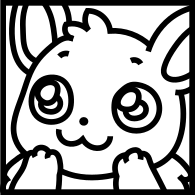
\includegraphics[height=2.5ex]{iibui.png}}}
\def\eeveeKawaii{\copy\eeveebox}

\NewTColorBox{proposition}{m}{
  standard jigsaw,
  sharp corners,
  boxrule=0.4pt,
  coltitle=black,
  colframe=black,
  opacityback=0,
  opacitybacktitle=0,
  fonttitle=\normalfont\bfseries\upshape,
  fontupper=\normalfont\itshape,
  title={Proposition #1},
  after title={.},
  attach title to upper={\ },
}

\renewcommand\qedsymbol{$\eeveeKawaii$}

\title{Hammack Exercises - Chapter 6}
\author{FungusDesu}
\date{September 6st 2024}

\begin{document}

\maketitle

\section{Preface}
i dont really have anything to say

\section{Section A - Proof by contradiction only}

\begin{proposition}{6.1}
    Suppose $n\in\mathbb Z$. If $n$ is odd, then $n^2$ is odd.
\end{proposition}

\begin{proof}
    Suppose for the sake of contradiction that $n$ is odd and $n^2$ is even. Then there exist $x,y\in\mathbb Z$ such that $n = 2x + 1$ and $n^2 = 2y$. Thus we have $4x^2+4x+1 = 2y$ implies $1 = 2(-2x^2 - 2x + y)$. Since $-2x^2 - 2x +y\in\mathbb Z$, we have $1$ is even, a contradiction.
\end{proof}

\begin{proposition}{6.2}
    Suppose $n\in\mathbb Z$. If $n^2$ is odd, then $n$ is odd.
\end{proposition}

\begin{proof}
    Suppose for the sake of contradiction that $n^2$ is odd and $n$ is even. Then there exist $x, y\in\mathbb Z$ such that $n^2 = 2x + 1$ and $n=2y$. Thus we have $4y^2 = 2x + 1$ implies $1 = 2(2y^2-x)$. Since $2y^2-x\in\mathbb Z$, we have $1$ is even, a contradiction.
\end{proof}

\begin{proposition}{6.3}
    $\sqrt[3]{2}$ is irrational.
\end{proposition}

\begin{proof}
    Suppose for the sake of contradiction that $\sqrt[3]{2}$ is rational. Then there exist $a,b\in\mathbb Z$ such that $\sqrt[3]{2} = \frac a b$. Let $\frac a b$ be irreducible; it follows that
    \begin{align}
        2b^3 = a^3,
    \end{align}
    which makes $a^3$ an even number. Thus $a$ must be even; because $a$ and $b$ cannot be both even, we have $b$ is odd. Since $a$ is even, there exist $c\in\mathbb Z$ such that $a = 2c$. Substituting that into Equation (1), we get $b^3 = 2(2c^3)$. Therefore $b^3$ is an even number, which implies $b$ is even. Thus we have a contradiction that $b$ is both odd and even.
\end{proof}

\begin{proposition}{6.4}
    $\sqrt6$ is irrational.
\end{proposition}

\begin{proof}
    Suppose for the sake of contradiction that $\sqrt6$ is rational. Then there exist $a,b\in\mathbb Z$ such that $\sqrt6=\frac a b$. Let $\frac a b$ be irreducible; it follows that
    \begin{align}
        a^2 = 2(3b^2),
    \end{align}
    which makes $a^2$ an even number. Thus $a$ must be even; because $a$ and $b$ cannot be both even, we have $b$ is odd. Since $a$ is even, there exist $c\in\mathbb Z$ such that $a = 2c$. Substituting that into Equation (2), we get $2c^2 = 3b^2$. Therefore $3b^2$ is even, which implies $b$ is even. Thus we have a contradiction that $b$ is both odd and even.
\end{proof}

\begin{proposition}{6.5}
    $\sqrt3$ is irrational.
\end{proposition}

\begin{proof}
    Suppose for the sake of contradiction that $\sqrt3$ is rational. Then there exist $a, b\in\mathbb Z$ such that $\sqrt3 = \frac a b$. Let $\frac a b$ be irreducible; it follows that 
    \begin{align}
    a^2 = 3b^2,
    \end{align}
    implying $3\mid a^2$. Because $3$ is prime and divides $a^2$, it follows that $a$ must contain $3$ in its prime factorization, thus $3 \mid a$. Therefore $a = 3x$ for some $x\in\mathbb Z$. Substituting it into Equation (3), we yield $b^2 = 3x^2$. Similarly, we can also conclude that $3\mid b$. Thus it is a contradiction that $a$ and $b$ share a common divisor of 3 when $\frac a b$ is irreducible.
\end{proof}

\begin{proposition}{6.6}
    If $a, b\in\mathbb Z$, then $a^2-4b-2\neq0$.
\end{proposition}

\begin{proof}
    Suppose for the sake of contradiction that $a^2-4b-2 = 0$ for some $a, b\in\mathbb Z$. Then we have $a^2=2(2b - 1)$, which implies $a^2$ is even. Thus $a$ is even and can be expressed as $a = 2k$ for some $k\in\mathbb Z$. Substituting that into the original equation, we get $2k^2 - 2b -1 = 0$ implies $1 = 2(k^2 - b)$. Therefore it is a contradiction that $1$ is an even number.
\end{proof}

\begin{proposition}{6.7}
    If $a, b\in\mathbb Z$, then $a^2-4b-3\neq0$.
\end{proposition}

\begin{proof}
    Suppose for the sake of contradiction that $a^2-4b-3=0$ for some $a, b\in\mathbb Z$. Then we have $a^2 = 2(2b-2)+1$, which implies $a^2$ is odd. Thus $a$ is odd and can be expressed as $a = 2k+1$ for some $k\in\mathbb Z$. Substituting that into the original equation, we yield $2k^2+2k-2b-1=0$ implies $1 = 2(k^2+k-b)$. Therefore it is a contradiction that $1$ is an even number.
\end{proof}

\begin{proposition}{6.8}
    Suppose $a,b,c\in\mathbb Z$. If $a^2+b^2=c^2$, then $a$ or $b$ is even.
\end{proposition}

\begin{proof}
    Suppose for the sake of contradiction that there exist odd $a$ and $b$ such that $a^2+b^2=c^2$ for some $c\in\mathbb Z$. Since $a$ and $b$ is odd, we have $a = 2m + 1$ and $b = 2n + 1$ for some $m,n\in\mathbb Z$. Substituting those into the original equation, we yield 
    \begin{align}
        4m^2 + 4m + 4n^2 + 4n + 2 = c^2\\
        c^2 = 2(2m^2 + 2m + 2n^2 + 2n + 1),
    \end{align}
    implying $c^2$, and consequently $c$, is even. Thus $c = 2k$ for some $k\in\mathbb Z$; substituting that into Equation (5) yields
    \begin{align*}       
        2k^2 = 2m^2 + 2m + 2n^2 + 2n + 1\\
        1 = 2(k^2 - m^2 - m - n^2 - n).
    \end{align*}
    Thus it is a contradiction that $1$ is even.
\end{proof}

\begin{proposition}{6.9}
    Suppose $a, b,\in\mathbb R$. If $a$ is rational and $ab$ is irrational, then $b$ is irrational.
\end{proposition}

\begin{proof}
    Suppose for the sake of contradiction that $a, b$ is rational and their product is irrational. Then $a = \frac{m_a}{n_a}$ and $b=\frac{m_b}{n_b}$ for some $m_a,n_a,m_b,n_b\in\mathbb Z$. Thus $ab = \frac{m_am_b}{n_an_b}$, contradicting the fact that $ab$ is irrational.
\end{proof}

\begin{proposition}{6.10}
    There exist no integers $a$ and $b$ for which $21a + 30b = 1$.
\end{proposition}

\begin{proof}
    Suppose for the sake of contradiction that there exist $a,b\in\mathbb Z$ such that $21a + 30b = 1$. Then $7a + 10b = \frac13$. Thus it is a contradiction that the sum of two integers is a non-integer.
\end{proof}

\begin{proposition}{6.11}
    There exist no integers $a$ and $b$ for which $18a+6b=1$.
\end{proposition}

\begin{proof}
    Suppose for the sake of contradiction that there exist $a, b\in\mathbb Z$ such that $18a + 6b = 1$. Then $3a + b = \frac16$. Thus it is a contradiction that the sum of two integers is a non-integer.
\end{proof}

\begin{proposition}{6.12}
    For every positive $x\in\mathbb Q$, there is a positive $y\in\mathbb Q$ for which $y<x$.
\end{proposition}

\begin{proof}
    Suppose for the sake of contradiction that there exists a positive $x \in\mathbb Q$ such that for all positive $y\in\mathbb Q$, we have $y\ge x$. At $y = \frac{x}{2}$, we have $0 < y < x$. Thus it is a contradiction that $y \ge x$ and $y < x$.
\end{proof}

\begin{proposition}{6.13}
    For every $x\in\left[\frac\pi2,\pi\right]$, $\sin x-\cos x\ge 1$.
\end{proposition}

\begin{proof}
    Suppose for the sake of contradiction that there exists $x\in\left[\frac\pi2,\pi\right]$ for which $\sin x-\cos x<1$. Since $x\in\left[\frac\pi2,\pi\right]$, we have $\sin x \ge 0$ and $\cos x\le 0$; consequently, their product is never positive. Thus we have:
    \begin{align*}
        0\le\sin x-\cos x<1.
    \end{align*}
    Squaring each side of the inequality, we obtain:
    \begin{align*}
        0\le\sin^2x-2\sin x\cos x+\cos^2x<1\\
        0<\sin x\cos x\le\frac12.
    \end{align*}
    Thus we have a contradiction.
\end{proof}

\begin{proposition}{6.14}
    If $A$ and $B$ are sets, then $A\cap (B-A)=\varnothing$.
\end{proposition}

\begin{proof}
    Suppose for the sake of contradiction that $A\cap(B-A)\neq\varnothing$ for some sets $A, B$. Then there exists $x\in(A\cap(B-A))$ and so $x\in A\land(x\in B \land x\notin A)$. Thus it is a contradiction that there exists an element that both belongs to $A$ and not belongs to $A$.
\end{proof}

\begin{proposition}{6.15}
    If $b\in\mathbb Z$ and $b\nmid k$ for every $k\in\mathbb N$, then $b = 0$.
\end{proposition}

\begin{proof}
    Suppose for the sake of contradiction that there exists an integer $b\neq 0$ such that $b\nmid k$ for all $k\in\mathbb N$. Then $b\mid |b|$; thus contradicting the fact that it does not divide any natural number.
\end{proof}

\begin{proposition}{6.16}
    If $a$ and $b$ are positive real numbers, then $a+b\ge2\sqrt{ab}$.    
\end{proposition}

\begin{proof}
    Suppose for the sake of contradiction that $a+b<2\sqrt{ab}$ for positive real $a$ and $b$. Then we have:
    \begin{align*}
        (a+b)^2 < 4ab\\
        a^2 + 2ab + b^2 < 4ab\\
        a^2 - 2ab + b^2 < 0\\
        (a-b)^2 < 0.
    \end{align*}
    Because $a-b\in\mathbb R$, it is a contradiction that the square of a real number is negative.
\end{proof}

\begin{proposition}{6.17}
    For every $n\in\mathbb Z$, $4\nmid (n^2+2)$.
\end{proposition}

\begin{proof}
    Suppose for the sake of contradiction that $4\mid n^2+2$ for some $n\in\mathbb Z$. Then there exists $x\in\mathbb Z$ such that $n^2 = 4x-2$. As proven in \textbf{Proposition 5.28}, because only $n^2\equiv 0\pmod4$ or $n^2\equiv1\pmod4$ is true and $(4x-2)\equiv2\pmod4$, it is contradictory that $n^2\equiv2\pmod4$.
\end{proof}

\begin{proposition}{6.18}
    Suppose $a,b\in\mathbb Z$. If $4\mid(a^2+b^2)$, then $a$ and $b$ are not both odd.
\end{proposition}

\begin{proof}
    Suppose for the sake of contradiction that if $4\mid(a^2+b^2)$, then $a$ and $b$ are both odd. Then $a = 2m+1$ and $b = 2n+1$ for some $m,n\in\mathbb Z$. Thus we have 
    \begin{align*}
        4\mid((2m+1)^2+(2n+1)^2)\\
        4\mid(4(m^2+m+n^2+n)+2).
    \end{align*}
    Therefore we have a contradiction.
\end{proof}

\section{Section B - Direct, contrapositive and contradiction}

\begin{proposition}{6.19}
    The product of any five consecutive integers is divisible by $120$.
\end{proposition}

\begin{proof}
    Consider any given five consecutive numbers. Notice that among them, \begin{itemize}
        \item there is always one number divisible by 5,
        \item there are at least two numbers divisible by 2, one of which is also divisible by 4,
        \item there is at least one number divisible by 3.
    \end{itemize}
    The multiples of 2 contribute 2 and 4 as the factors, multiples of 3 contribute 3 and multiple of 5 contributes 5. And because $2\cdot3\cdot4\cdot5=120$, it is evident their product is always a multiple of 120, as desired.
\end{proof}

\begin{proposition}{6.20}
    The curve $x^2+y^2-3=0$ has no rational points.
\end{proposition}

\begin{proof}
    Suppose for the sake of contradiction that there exists a rational point in the curve $x^2 + y^2 - 3 = 0$. Let $P=(x_0, y_0)$ be such rational point; then $x_0 = \frac{m}{q}$ and $y_0 = \frac{n}{q}$ for some $m,n,q\in\mathbb Z$. Substituting $P$ into the curve, we obtain:
    \begin{align*}
        \frac{m^2}{q^2}+\frac{n^2}{q^2} = 3\\
        m^2+n^2 = 3q^2.
    \end{align*}
    We define the \textbf{$p$-adic valuation} of a non-zero integer $n$ to be the highest exponent of the prime number $p$ in the factorization of $n$, denoted as $v_p(n)$. Thus \[
        v_p(n) = \max(\{k\in\mathbb N: p^k\mid n\}).
    \]
    Let $a, b, c$ be the 3-adic valuation of $m^2, n^2$ and $q^2$ respectively. Let $z^2$ and $w^2$ be arbitrary square numbers. To complete the proof, we shall show that $v_3(z^2+w^2) = \min(v_3(z^2), v_3(w^2))$. We divide into two cases as follow:
    \begin{description}
        \item[Case 1. ] If $v_3(z^2)\neq v_3(w^2)$, then
        \begin{align*}
            &v_3(z^2+w^2)\\
            &= v_3(2^{v_2(z^2)}\cdot3^{v_3(z^2)}\cdot5^{v_5(z^2)}\cdots+2^{v_2(w^2)}+3^{v_3(w^2)}+5^{v_5(w^2)}\cdots)\\
            &= v_3(3^{\min(v_3(z^2), v_3(w^2))}\cdot(2^{v_2(z^2)}\cdot3^{v_3(z^2)-\min(v_3(z^2), v_3(w^2))}\cdot5^{v_5(z^2)}\cdots\\
            &+2^{v_2(w^2)}+3^{v_3(w^2 - \min(v_3(z^2), v_3(w^2)))}+5^{v_5(w^2)}\cdots)).
        \end{align*}
        Because factoring $3^{\min(v_3(z^2),v_3(w^2))}$ leaves the sum with exactly 1 term divisible by 3, the sum is no longer a multiple of 3. Thus by definition, $v_3(z^2+w^2) = \min(v_3(z^2), v_3(w^2))$.
        \item[Case 2. ] If $v_3(z^2)= v_3(w^2)$, we use the same process of reduction in \textbf{Case 1} to reduce the sum into one where both terms are not divisible by 3. Here we consider the divisibility of 3 on the sum itself. Because only either $a^2\equiv0\pmod3$ or $a^2\equiv1\pmod3$ is true for arbitrary integer $a$, if $a^2$ is not divisible by 3, then only $a^2\equiv1\pmod3$ is true. Thus $(\frac{z^2}{3^{v_3(z^2)}} + \frac{w^2}{3^{v_3(w^2)}})\equiv2\pmod3$. By the same principle in \textbf{Case 1}, it is also true in this case that $v_3(z^2+w^2)=\min(v_3(z^2),v_3(w^2))$.
    \end{description}
    Thus $m^2+n^2=3q^2$ is a sufficient condition for $v_3(m^2+n^2) = v_3(3q^2)$, which implies $\min(a, b) = c + 1$. On the other hand, observe that $a, b, c$ must all be even since all the terms' powers in their prime factorizations are even. Thus $\min(a,b)$ and $c + 1$ have opposite parity, implying they cannot be equal. Therefore we have a contradiction.
\end{proof}

\begin{proposition}{6.21}
    $\sqrt3$ is irrational because the curve $x^2 + y^2 - 3 = 0$ has no rational points.
\end{proposition}

\begin{proof}
    Consider the case where $(x,y) = (q, 0)$ is a point on the curve $x^2+y^2-3 = 0$. Thus we have $q^2 = 3$ implies $q = \sqrt3$. As proven in \textbf{Proposition 6.20} that the curve $x^2+y^2-3 = 0$ has no rational points, $q$ and 0 must not be both rational. 0 is rational, thus $q = \sqrt3$ is irrational, and we are done.
\end{proof}

\begin{proposition}{6.22}
    $x^2+y^2-3=0$ not having any rational solutions implies $x^2 + y^2-3^k=0$ has no rational solutions for $k$ an odd, positive integer.
\end{proposition}

\begin{proof}
    Becuase $k$ is odd, we have $x^2 + y^2=3^{2n + 1}$ for some integer $n$. Dividing both sides by $3^{2n}$ yields $\frac{x^2}{3^{2n}}+\frac{y^2}{3^{2n}}=3$. Let $u = \frac{x}{3^n}$ and $v = \frac{y}{3^n}$, we see that $u$ and $v$ are rational if and only if $x$ and $y$ are rational. As such, we can form a bijection between the rational solutions of $\left(\frac{x}{3^n}\right)^2 + \left(\frac{y}{3^n}\right)^2 = 3$ and $u^2 + v^2 = 3$. However, \textbf{Proposition 6.20} says the latter has no rational solutions. Therefore neither does the former.
\end{proof}

\begin{proposition}{6.23}
    $\sqrt{3^k}$ is irrational for all odd, positive $k$.
\end{proposition}

\begin{proof}
    Consider the case where $(x,y) = (q, 0)$ is a point on the curve $x^2+y^2-3^k = 0$. Thus we have $q^2 = 3^k$ implies $q = \sqrt{3^k}$. As proven in \textbf{Proposition 6.22} that the curve $x^2+y^2-3^k = 0$ has no rational points for positive odd $k$, we have $q$ and 0 must not be both rational. 0 is rational, thus $q = \sqrt{3^k}$ is irrational, and we are done.
\end{proof}

\begin{proposition}{6.24}
    The number $\log_23$ is irrational.
\end{proposition}

\begin{proof}
    Suppose for the sake of contradiction that $\log_23$ is rational. For the sake of simplicity, there exist $m,n\in\mathbb Z$ such that $\log_23 = \frac m n$, and $m, n>0$ since the fraction is positive ($\log_23$ is positive because $\log_23>\log_22=1$). Let this fraction be irreducible; thus $3 = 2^{\frac m n}$, implying $3^n = 2^m$. For all $m, n\in\mathbb Z_{>0}$, we can see that $3^n$ is always odd, while $2^m$ is always even. Thus it is a contradiction that two numbers of opposite parity are equal.
\end{proof}

\end{document}